\section{Om equalizers}\label{sec:equalizer}

En equalizer er et form for filter der har til formål at udglatte eller ændre et givent signal. I modsætning til filtre der normalt designes til et specifikt formål er equalizeren justerbar og kan tilpasses alt afhængig af det signal der påtrykkes og hvilket formål der ønskes.\\

Der er to hovedgrupper af equalizers: Grafiske equalizere og parametriske equalizere.\\
Der er uenighed i definitionerne af de to typer, hvilket medfører forvirring omkring specifikationer af filter. I denne rapport vælges følgende definitioner:

\begin{itemize}
	\item Grafisk equalizer\footnote{Screenshot fra iTunes Equalizer, figur \ref{fig:graphic_eq} \url{http://www.apple.com/itunes}}: Her splittes equalizeren op i forskellige bånd der dækker sine fastlagte frekvens områder. Som bruger har man forstærkning af det respektive bånd som parameter at ændre på. Båndbredde og center frekvens er fastlagt.
	\item Parametrisk equalizer \footnote{Screenshot fra Ableton Live, figur \ref{} \url{http://www.ableton.com}}: Her er båndene vilkårlige således, at brugeren selv kan tilføje og fjerne dem efter behov. I hvert enkelt bånd kan man justere båndbredde, center frekvens og forstærkning ved center frekvensen. Alt efter computer / mikrocontroller er der dog et maksimum antal bånd da equalizeren ellers vil kræve for meget CPU kraft. 
\end{itemize}  

\begin{figure}[h]
	\centering
	\subbottom[]{%
	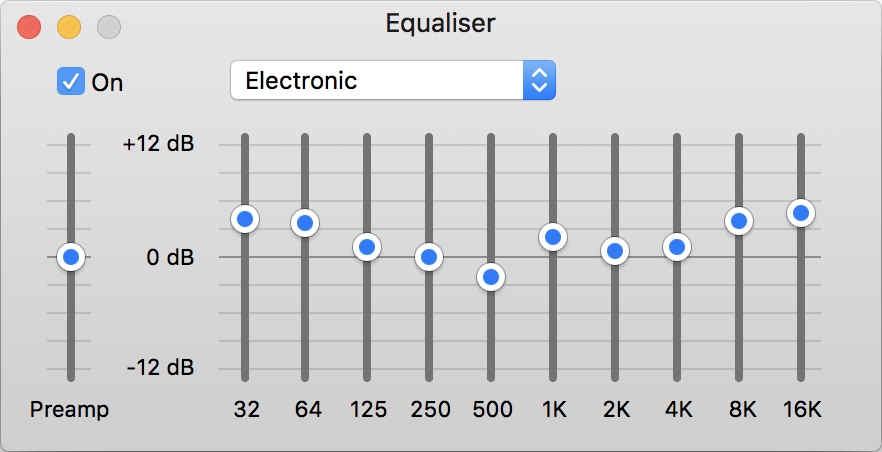
\includegraphics[width=7cm]{billeder/graphic_eq}
	\label{fig:graphic_eq}}
	\subbottom[]{%
	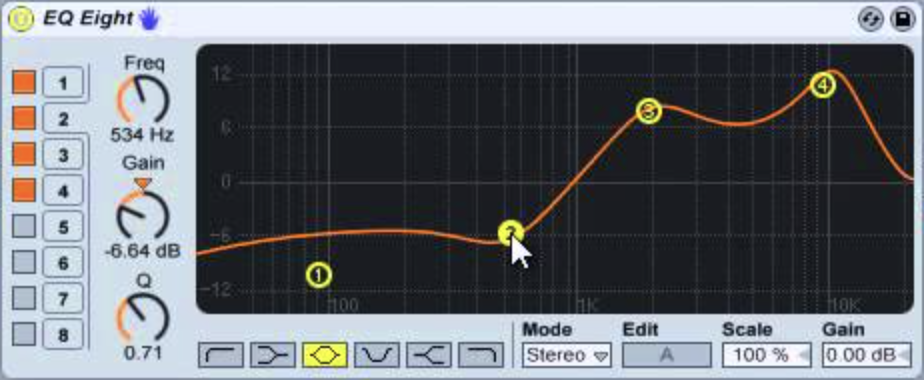
\includegraphics[width=7cm]{billeder/parametric_eq}
	\label{fig:parametric_eq}}
  	\caption{(a) Eksempel på GUI til en grafisk equalizer, (b) Eksempel på GUI til en parametrisk equalizer.}
	\label{fig:om_eq}
\end{figure}
\FloatBlock

Af de to equalizer typer, er den parametriske klart den mest fleksible men også den mere beregningstunge. På figur \ref{fig:om_eq} kan der tydeligt ses forskel. F.eks. har den parametriske equalizer (figur \ref{fig:parametric_eq}) nogle frekvens specifikationer som den grafiske equalizer ikke kan realisere.\\

Equalizere bruges mange steder hvor lydens "kvalitet" er vigtig. 
De bruges f.eks. i studio teknik, radio teknik, telefoni, forbruger-lydforstærkerer og til koncerter. 
Til de forskellige applikationer er der forskellige ind- og udgangsniveauer som skal overholdes. 
I professionel lyd er linje-signalet f.eks. højere end ved normal forbruger lyd. 